\documentclass[11pt,a4paper,notitlepage]{article}

%usepackage inclusions:
\usepackage{mathtools} %package that allows math formatting
\usepackage{commath} %package that allows for nice differential operators
\usepackage{bigints} %package that allows for bigger integral signs
\usepackage{amsfonts}   %package that allows for more math characters
\usepackage{amssymb}  %package that allows for more math symbols
\usepackage{shadethm}  %package that allows for shaded definitions&proofs
\usepackage[usenames,dvipsnames,svgnames,table]{xcolor} %package that allows colored text
\usepackage{booktabs}
\usepackage{float} % by Jakob
\usepackage{graphicx}
\usepackage[table]{xcolor} %to color table rows & columns
\usepackage{setspace} %to allow for the insertion line spaces at will
\usepackage{wrapfig} %to allow for figures to be captioned
\usepackage{mdframed} % to allow for wide frames and boxes around math&text
\usepackage[makeroom]{cancel} %to allow for strike-out text
\usepackage{subfigure}
\usepackage{parskip}
\usepackage{url} %to allow citing url addresses
\usepackage{rotating}
\usepackage{nameref}
\usepackage{geometry}
\usepackage[margin=1cm]{caption}
\usepackage{changepage}
\usepackage{natbib}
\usepackage{titlesec}

\setcounter{secnumdepth}{4}
\setcounter{tocdepth}{4}

\titleformat{\paragraph}
{\normalfont\normalsize\bfseries}
{\theparagraph}{1em}{}

\titlespacing*{\paragraph}
{0pt}{3.25ex plus 1ex minus .2ex}{1.5ex plus .2ex}

%define own operators&theorems&proofs
\newcommand{\expect}[1]{\mathbb{E} \left[ {#1} \right] } %define expectation symbol 
\newtheorem{proof}{Proof} %define proofs within the shadethm environment
\newcommand{\vect}[1]{\boldsymbol{#1}} %define  BOLD vectors.
\newcommand{\expe}[1]{\mathbb{E}\left[#1\right]} %define  BOLD vectors.
\newcommand{\HRule}{\rule{\linewidth}{0.01mm}} %define horizontal thin line
\newcommand{\red}[1]{{\color{red}{#1}}}

%set page margins
%\addtolength{\textheight}{2cm} 
%\addtolength{\voffset}{-1cm}
%\addtolength{\textwidth}{2cm}
%\addtolength{\hoffset}{-3cm}
\setlength{\oddsidemargin}{0pt} %set left & right margins
\setlength{\evensidemargin}{0pt} %set left & right margins
%set headers and footers
%\usepackage{fancyhdr}  
%\setlength{\headheight}{0pt}
%\pagestyle{fancy}
%\fancyhf{}
\usepackage{indentfirst}
\numberwithin{equation}{section}
%set fonts used
%\usepackage{lmodern}
%\usepackage{kpfonts}
%can check http://www.tug.dk/FontCatalogue/mathfonts.html for font alternatives
%set authoring details
\author{ %name under title %email in footnote \thanks{a.lalu@tinbergen.nl} 
	    }
\title{\vspace*{-55pt} Risk Premium Inference from (Noisy) Option Price Panels \vspace*{-35pt}}
\date{\item First version: June 16, 2018 \item Previous Version : May 20, 2026 \item This version: \today}
%start file content
\begin{document}
\maketitle
%\abstract{
%\tableofcontents
%}

\onehalfspacing

\section*{Brief Description of Research Idea}
Compare the finite sample performance of implied state vs. particle filtering when conducting joint $\mathbb{P}$-$\mathbb{Q}$	estimation on noisy option price panels focusing on the implications this has for recovered (equity) risk premium components and their error distributions/confidence bands. 

\section*{Tentative Outline of Building Blocks}
\begin{enumerate}
\item Implement an efficient simulation scheme for a Heston \citep{heston} state space simulation and associated option price panels.
\item Implement IS estimation \`{a} la \cite{boswijk2015asset}.
\item Implement particle filtering \`{a} la \cite{hurn2015pf}.
\item No noise/best case.
\item Noisy option panel case with an assorted menu of assumptions regarding option price error distributions.
\end{enumerate}

\section*{Rationale}
\begin{enumerate}
\item[A.] Noisy option data is something I had to deal with both for the first two papers, outside academia and having spent some more time looking at post 2018 academic work it seems that this is an emerging topic with a few papers that touch on this in a different context: \cite{andersen2021spatial}, \cite{duarte2024very}.
\item[B.] Topic itself ties in well with the other two papers in my thesis.
\item[C.] I have sufficient background to work on this independently.
\end{enumerate}

\newpage
 
\section{Assumed Data Generating Proces And Option Pricing}
We consider a filtered probability space $\left(\Omega, \mathcal{F}, \lbrace\mathcal{F}\rbrace_{t\geq0}, \mathbb{P} \right)$ satisfying the usual conditions\footnote{See e.g., \citet{protterstochastic}, p. 3.}. Under the historical probability measure, $\mathbb{P}$, the dynamics of the log-price process $\log(S_t)$ and of the stochastic volatility process $V_t$, which make up the state vector $X_t = [\log(S_t), V_t]$, are assumed to be described by the pair of s.d.e.:
\begin{align}
	\dif{\log(S_t)} &= \left((r_t-q_t)+ \left(\eta-1/2\right) V_t \right)\dif t + \sqrt{V_t} \dif W_{t,1}^\mathbb{P}; \label{PHestonS}\\
	\dif{V_t} &= k(\bar{V}-V_t)\dif t + \sigma_v\sqrt{V_t}\left(\rho \dif W_{t,1}^\mathbb{P} + \sqrt{1-\rho^2}\dif W_{t,2}^\mathbb{P}\right). \label{PHestonV}
\end{align}
$\left(\dif W_{t,1}^\mathbb{P}, \dif W_{t,2}^\mathbb{P}\right)$ are $\mathcal{F}_t$-adapted Brownian motion processes. $\lbrace r \rbrace_{t\geq 0}$  and  $\lbrace q \rbrace_{t\geq 0}$ are $\mathcal{F}_t$-adapted processes (e.g., deterministic) which describe the risk-free rate of interest and the continuous dividend yield respectively. $\eta$ is a parameter which governs the size of the equity risk premium. The local stochastic volatility process mean reverts at a mean reversion rate $\kappa$ to the long run mean level $\bar{V}$. $\sigma_v$ governs the volatility of volatility and $\rho$ represents the instantaneous correlation between returns and volatility.

Under the risk neutral probability measure, $\mathbb{Q}$, the model dynamics are assumed to be: 
\begin{align}
	\dif{\log(S_t)} &= \left( (r_t-q_t) - 1/2 V_t\right) \dif t + \sqrt{V_t} \dif W_{t,1}^\mathbb{Q};\label{QHestonS}\\
	\dif{V_t} &= k(\bar{V}-V_t)\dif t + \eta_{V}V_t\dif t + \sigma_v\sqrt{V_t}\left(\rho \dif W_{t,1}^\mathbb{Q} + \sqrt{1-\rho^2}\dif W_{t,2}^\mathbb{Q}\right).\label{QHestonV}
\end{align}
$\left(\dif W_{t,1}^\mathbb{Q}, \dif W_{t,2}^\mathbb{Q}\right)$ are Brownian motions under the (equivalent) martingale pricing measure $\mathbb{Q}$.

Jointly, \ref{QHestonS} and \ref{QHestonV} are known as the Heston model, which features local stochastic volatility with a leverage effect while providing semi-closed form solutions for option prices. This model is a "staple" stochastic volatility model for equity index modeling. It is used in a large number of empirical studies, has a number of well documented limitations, some of which have been remedied by enriching the model specification through the addition of jumps and/or other (latent) stochastic states. 

Given the focus of the study, attention is restricted to the simplistic set-up of the Heston model for a host of reasons. On the one hand, for most Heston model extensions, econometric approaches to parameter estimation which employ option price data come with increased computational costs. Since in the current set-up this model is known to be the data generating process, there's no potential misspecification issue at play.
Secondly, extensions come with specific estimation challenges which typically require tailored estimation designs to obtain well-behaved parameter estimates therefore limiting the comparability of results obtained throughout the study. 

\subsection{Parameter Sets}
Let $\theta$ denote the vector of parameters featured in the model. We assume $\theta \in \Theta$ where $\Theta$ is a compact set from the domain of valid data-generating process parameters. For the Heston model specification previously introduced, the value of $\theta$ corresponding to the data-generating process introduced in \eqref{PHestonS} - \eqref{QHestonV} is $\theta = \left[\eta, \kappa, \bar{v}, \sigma_v, \rho, \eta_v\right]$. Note that subsets of the parameter set play a role in either the $\mathbb{P}$-measure specification, the $\mathbb{Q}$-measure specification or in both. E.g., the Heston parameter set can be decomposed into 3 disjoint subsets: $\theta = \left[\theta^\mathbb{P}, \theta^{\mathbb{P}\cap\mathbb{Q}}, \theta^\mathbb{Q}\right]$, where $\theta^\mathbb{P} = \eta$,~ $\theta^{\mathbb{P}\cap\mathbb{Q}} = \left[\kappa, \bar{v}, \sigma_v, \rho\right]$, and $\theta^\mathbb{Q} = \eta_v$. 

\subsection{State Vector}
Assuming we have a time series of state vector observations:\footnote{In practice such a series never exists as the volatility, $V_t$, is an unobservable, i.e., latent state process} $X_1, \dots, X_T$, observed at  equally-spaced timepoints $t_1,\dots,t_T$ with $t_{i+1} - t_i = \Delta >0, \forall i\geq 1 $. Denote by $f(X_{i+1} |X_i; \theta^\mathbb{P},  \theta^{\mathbb{P} \cap \mathbb{Q}})$ the transition density of the state vector $X_t$ under the historical probability measure. Note that the transition density depends on $\theta^\mathbb{P}$ and $\theta^{\mathbb{P} \cap \mathbb{Q}}$ which represent the subset of parameters that describe the model dynamics under $\mathbb{P}$.

By using option price data the full set of parameters -- including the additional ones that characterize model dynamics under the risk neutral pricing measure -- can be estimated, i.e., inference on $\theta^\mathbb{Q}$ can be conducted while at the same time increasing sample identification potential for the $\theta^{\mathbb{P} \cap \mathbb{Q}}$ parameter set. 

\subsection{Option prices}
Suppose that, in addition to time series observations of returns, synchronous observations of option price panel data and time series data on the underlying are available. Denote the option prices by $p_{i}(T,K)$ where $T,K$ represent the maturity and the strike of the option contract. Option prices are commonly quoted in terms of their Black-Scholes implied volatility. Let $P(X_{i},T,K; \theta^{\mathbb{P}\cap\mathbb{Q}}; \theta^\mathbb{Q})$ be the corresponding model price, e.g., the option price generated by the base model specification under the equivalent martingale pricing measure for  given state vector instance $X_{i}$ and parameter set values $\theta^{\mathbb{P}\cap\mathbb{Q}}$ and $\theta^\mathbb{Q}$. If option prices were observed without error and the model is not misspecified, the observed option prices would coincide with their model-based counterparts. In practice the two prices differ. Typical modelling approaches assume away model misspecification and attribute the difference to measurement errors (e.g., microstructure noise).  This assumption can in practice have consequences for the sample properties of the estimator of choice and thus warrants further consideration.

\subsubsection{Option Prices with Observation Errors}
Suppose that, at each observation date $t_i$, a panel of option price quotes is observed for a set of contracts from ranging from $j=1$ to $j=q_i$ where $q_i \in \mathbb{N}^*$. This set is denoted by $\mathcal{C}_i=\{(T_i^{(j)},K_i^{(j)})\}_{j=1}^{q_i}$ and the resulting price vector by
$p_i^{\mathrm{obs}}=\left(p_i^{(1),\mathrm{obs}},\dots,p_i^{(q_i),\mathrm{obs}}\right)^\top$, where $p_i^{(j),\mathrm{obs}}=p_i^{\mathrm{obs}}(T_i^{(j)},K_i^{(j)})$ is the observed price for option contract $j$.


Similarly, let $p_i^{0}=p_i^{\mathrm{model}}=\left(p_i^{(1),0},\dots,p_i^{(q_i),0}\right)^\top$
be the vector of corresponding model-based prices implied by
$P(X_i,T,K;\theta^{\mathbb{P}\cap\mathbb{Q}};\theta^\mathbb{Q})$. Let $\sigma_i^{0} = \left(\sigma_i^{(1),0},\dots,\sigma_i^{(q_i),0}\right)^\top$ denote the corresponding Black-Scholes implied volatility vector.

The difference between $p_i^{\mathrm{obs}}$ and $p_i^{\mathrm{model}}$ is interpreted as option observation error.
This difference can be, inter alia, attributed to microstructure effects, stale quotes or price discreteness due to minimum tick sizing or quote rounding conventions. \citet{duarte2024very}
suggests that such frictions can be quantitatively important for inference involving option-implied risk premia. 

The proposed simulation design therefore does not commit ex-ante to a single parametric error law but instead considers three observed-panel specifications generated from the same clean model-implied panel. Each specification is meant to reflect empirical concerns raised by the recent literature while keeping the data generating exercise tractable. The three specifications are introduced in implied-volatility space. The corresponding noisy prices are then obtained through the Black-Scholes pricing formula, rounded to the relevant tick size and projected back into the no-arbitrage price interval. This keeps the treatment of all three observation error specifications internally consistent while preserving both price and implied-volatility representations of the noisy option panel.

\paragraph{Design A: Low I.I.D. noise}
First, a low-noise benchmark is introduced in which observation errors are independent across contracts, but the marginal scale of the error is allowed to vary with moneyness and maturity. This reflects the fact that option observation errors need not have the same relative impact across the surface and can enter the behaviour of option-based estimators through local features of the panel, in particular for contracts close to the spot or forward price as discussed in \cite{chongtodorov2024vov}.
For $j=1,\ldots,q_i$, let
\[
m_i^{(j)}=\log\left(\frac{K_i^{(j)}}{F_i^{(j)}}\right),
\qquad
\mathcal T_i^{(j)}=T_i^{(j)}-t_i,
\]
where $F_i^{(j)}$ denotes the corresponding forward price. The marginal implied-volatility observation error scale is specified as
\begin{align}
s_{\sigma,i}^{(j)}
=
s_\sigma(m_i^{(j)},\mathcal T_i^{(j)})
=
\alpha_0\left(
1+\alpha_m |m_i^{(j)}|
+\frac{\alpha_{\mathcal T}}{\sqrt{\max(\mathcal T_i^{(j)},\mathcal T_{\min})}}
\right).
\label{eq:iv_error_scale}
\end{align}
The first specification is intended to mimic a liquid-market benchmark in which implied-volatility observation errors are independent across contracts conditional on the clean panel:
\begin{align}
\tilde\sigma_i^{(j),A}
=
\max\left\{
\sigma_{\min},
\sigma_i^{(j),0}
+
s_{\sigma,i}^{(j)}Z_i^{(j)}
\right\},
\qquad
Z_i^{(j)}\overset{i.i.d.}{\sim}\mathcal{N}(0,1).
\label{eq:noise_liquid}
\end{align}
In other words, this specification represents small quote observation errors whose scale varies with moneyness and maturity, without imposing dependence across contracts. It serves as the low-noise benchmark case.

The realised implications of the observation-error specifications are illustrated in Appendix~B. In the low i.i.d. design, the perturbations are contract-specific and preserve the broad shape of the clean implied-volatility panel, while allowing the local noise scale to vary with moneyness and maturity.

\paragraph{Design B: Cross-sectionally correlated noise}
A second observation error design allows for cross-sectional dependence in a given option panel for timepoint $t_i$ by correlating errors across nearby strikes and tenors. This is largely motivated by the evidence and testing framework in \cite{andersen2021spatial}, which explicitly considers spatial dependence in option observation errors. In this specification, the information content of a panel with $q_i$ option prices is essentially not equivalent to that of $q_i$ independent observations.

Let
$\varepsilon_i^B=\left(\varepsilon_i^{(1),B},\ldots,\varepsilon_i^{(q_i),B}\right)^\top$ and set
\begin{align}
\tilde\sigma_i^{(j),B}
=
\max\left\{
\sigma_{\min},
\sigma_i^{(j),0}
+
\varepsilon_i^{(j),B}
\right\},
\qquad
j=1,\ldots,q_i,
\label{eq:noise_spatial_iv}
\end{align}
where
\begin{align}
\varepsilon_i^B\sim\mathcal{N}(0,D_i R_i D_i),
\label{eq:noise_spatial}
\end{align}
with
\[
D_i=\mathrm{diag}\left(s_{\sigma,i}^{(1)},\ldots,s_{\sigma,i}^{(q_i)}\right).
\]
The correlation matrix $R_i$ is given by
\begin{align}
R_{i,jk}
=
\exp\left(
-\frac{|m_i^{(j)}-m_i^{(k)}|}{\ell_m}
-\frac{|\mathcal T_i^{(j)}-\mathcal T_i^{(k)}|}{\ell_{\mathcal T}}
\right).
\label{eq:spatial_kernel}
\end{align}
This specification captures the possibility that nearby strikes and maturities share common quote or surface construction errors.

The cross-sectionally correlated design creates locally coherent distortions across nearby moneyness and maturity points. Appendix~B reports the corresponding noisy option panels, signed perturbations and cross-sectional correlation structure.

\paragraph{Design C: Temporally persistent noise}
The third observation error design allows for a persistent common component in the observation error, affecting the level, moneyness slo1pe and maturity slope of the noisy implied volatility panel. This is consistent with the practical treatment of option panels as surfaces and with the broader evidence that option price noise can be quantitatively relevant for inference on risk premia as in \cite{duarte2024very}.

Let
$f_i=(f_{0,i},f_{1,i},f_{2,i})^\top$ evolve according to
\begin{align}
f_i=A f_{i-1}+\xi_i,
\qquad
\xi_i\sim\mathcal{N}(0,Q),
\label{eq:factor_noise}
\end{align}
where $A$ is diagonal with entries inside the unit circle. For contract $j$, define
\[
b_i^{(j)}
=
\left(1,m_i^{(j)},\mathcal T_i^{(j)}\right)^\top.
\]
The raw implied-volatility observation error is
\begin{align}
\tilde\sigma_i^{(j),C}
=
\max\left\{
\sigma_{\min},
\sigma_i^{(j),0}
+
\left(b_i^{(j)}\right)^\top f_i
+
u_i^{(j)}
\right\},
\qquad
u_i^{(j)}\sim\mathcal{N}\left(0,\left(s_{\sigma,u,i}^{(j)}\right)^2\right),
\label{eq:factor_iv_noise}
\end{align}
where $s_{\sigma,u,i}^{(j)}$ is allowed to depend on $m_i^{(j)}$ and $\mathcal T_i^{(j)}$. 

The matrix $A$ is the persistence matrix of the common observation-error factors. In the present specification it is taken to be diagonal, so that each component of $f_i$ follows a separate first-order autoregressive process. The restriction that the diagonal entries of $A$ lie inside the unit circle ensures stationarity. The matrix $Q$ is the covariance matrix of the innovations $\xi_i$ and controls the magnitude and possible co-movement of new shocks to the common components of the observation error.

The factor representation is a parsimonious way of introducing temporal dependence in the option panel observation errors. The vector $f_i$ describes the common observation-error state at date $t_i$, while the loading vector $b_i^{(j)}$ determines how this common component affects option contract $j$, i.e., $\left(b_i^{(j)}\right)^\top f_i = f_{0,i}+m_i^{(j)}f_{1,i}+\mathcal T_i^{(j)}f_{2,i}.$
The first component acts as a common level error, the second component as a moneyness-slope error, and the third component as a maturity-slope error. This type of low-dimensional factor representation is consistent with the empirical treatment of implied-volatility panels as objects whose movements can be summarised by a small number of common components; see, for example, \cite{cont2002dynamics} and related PCA-based evidence for implied-volatility surface such as  \cite{avellaneda2020pca}.

Compared to Designs A and B, the persistent-factor design C induces serially dependent quote distortions through (several) common component(s). Appendix~B reports the realised factor paths and their effect on representative option contracts.

For all three specifications, the raw noisy price is obtained from the Black-Scholes pricing function:
\begin{align}
\tilde p_i^{(j)}
=
B^{\mathrm{BS}}
\left(
S_i,K_i^{(j)},\mathcal T_i^{(j)},r_i,q_i,\tilde\sigma_i^{(j)}
\right).
\label{eq:raw_contaminated_price}
\end{align}
The raw noisy price $\tilde p_i^{(j),}$ is then rounded to the relevant tick size and projected back into the no-arbitrage price interval for the corresponding European option. The observed implied volatility $\sigma_i^{(j),\mathrm{obs}}$ is obtained by inverting the Black-Scholes pricing formula at the resulting observed price $p_i^{(j),\mathrm{obs}}$. This final step ensures that the noisy panel contains both observed prices and observed implied volatilities, and that invalid prices generated by the noise mechanism are handled by capping rather than by re-sampling.

The detailed calibration of the noise parameters and the contract design $\mathcal{C}_i$ are deferred to Appendix~\ref{app:option_noise_specs}.

Note that the three observation error specifications are written in terms of model prices and Black-Scholes implied volatilities. Black-Scholes vegas are stored alongside the generated panels so that the same noisy panels can also be used in vega-scaled estimation exercises if required.

\subsubsection{Implied-State C-GMM Estimation}
\label{sec:is_cgmm_estimation}

The first estimation approach considered in the Monte Carlo exercise is an implied-state continuum GMM estimator in the spirit of \citet{boswijk2015asset}. The estimator uses the option panel at each observation date to recover a parameter-dependent proxy for the latent variance state and subsequently imposes moment restrictions based on the conditional characteristic function of the resulting state vector. This provides a natural benchmark for the particle-filter approach introduced below. The implied-state estimator summarises each option panel by a latent state implied from the cross-section of option prices, whereas the particle filter treats the option panel as part of the measurement system used to update a distribution of latent states.

Let
\[
\theta_{\mathbb Q}
:=
\left[
\theta^{\mathbb{P}\cap\mathbb{Q}},
\theta^\mathbb{Q}
\right]
\]
denote the subset of parameters which enters the risk-neutral option pricing problem. In the Heston specification considered, this corresponds to
\[
\theta_{\mathbb Q}
=
\left[
\kappa,\bar V,\sigma_v,\rho,\eta_V
\right].
\]
Given a candidate value of \(\theta_{\mathbb Q}\), the observed option panel at date \(t_i\) can be used to construct an implied variance state. Let
\[
\sigma_i^{\mathrm{obs}}
=
\left(
\sigma_i^{(1),\mathrm{obs}},
\dots,
\sigma_i^{(q_i),\mathrm{obs}}
\right)^\top
\]
denote the vector of observed Black-Scholes implied volatilities corresponding to the contracts in \(\mathcal C_i\). For a candidate variance level \(v\), let
\(
\sigma^{(j),\mathrm{model}}
\left(
\log(S_i),v;\theta_{\mathbb Q}
\right)
\)
denote the model-implied Black-Scholes volatility of contract \(j\) obtained from the Heston pricing model. The implied variance state is defined as
\[
\widehat V_i^{\theta_{\mathbb Q}}
=
\arg\min_{v\in\mathcal V}
\sum_{j=1}^{q_i}
\left[
\sigma_i^{(j),\mathrm{obs}}
-
\sigma^{(j),\mathrm{model}}
\left(
\log(S_i),v;\theta_{\mathbb Q}
\right)
\right]^2 ,
\label{eq:is_implied_state}
\]
where \(\mathcal V\) is the admissible domain for the variance state. In the absence of observation error, and evaluated at the true parameter vector, this inversion recovers the latent variance sequence up to numerical approximation error. In noisy option panels, \(\widehat V_i^{\theta_{\mathbb Q}}\) is instead a parameter-dependent transformation of the noisy option cross-section. This is the main channel through which option observation errors affect the implied-state estimator.

Define the observed log-return increment
\[
R_i
:=
\log(S_i)-\log(S_{i-1})
\]
and collect the observable return and implied variance into the parameter-dependent estimation state:
\[
X_i^{\theta_{\mathbb Q}}
=
\left(
R_i,
\widehat V_i^{\theta_{\mathbb Q}}
\right)^\top .
\label{eq:is_state_vector}
\]
Although the state-implying step depends only on \(\theta_{\mathbb Q}\), the transition law of \(X_i^{\theta_{\mathbb Q}}\) under the historical probability measure depends on the full parameter vector \(\theta\). Let
\[
\varphi\left(s,X_i^{\theta_{\mathbb Q}},\Delta;\theta\right)
=
\mathbb E_\theta
\left[
\exp\left(
is^\top X_{i+1}^{\theta_{\mathbb Q}}
\right)
\mid X_i^{\theta_{\mathbb Q}}
\right]
\]
denote the conditional characteristic function of the next estimation state, where \(s\in\mathbb R^2\). For the Heston model this conditional characteristic function is available in affine form under \(\mathbb P\), since the dynamics of the return and variance pair are driven by the square-root variance process.

The implied-state C-GMM estimator is based on the martingale difference
\[
e_i(s;\theta)
=
\exp\left(
is^\top X_{i+1}^{\theta_{\mathbb Q}}
\right)
-
\varphi\left(s,X_i^{\theta_{\mathbb Q}},\Delta;\theta\right).
\label{eq:is_cgmm_error}
\]
Following the characteristic-function approach to GMM estimation, this residual is multiplied by a continuum of instruments of the form
\[
\exp\left(
iu^\top X_i^{\theta_{\mathbb Q}}
\right),
\qquad u\in\mathbb R^2 .
\]
Let \(\tau=(u,s)\) denote the combined argument of the continuum of moment conditions. The moment function is
\[
h_i(\tau;\theta)
=
\exp\left(
iu^\top X_i^{\theta_{\mathbb Q}}
\right)
\left[
\exp\left(
is^\top X_{i+1}^{\theta_{\mathbb Q}}
\right)
-
\varphi\left(s,X_i^{\theta_{\mathbb Q}},\Delta;\theta\right)
\right].
\label{eq:is_cgmm_moment}
\]
At the true parameter value, and under the maintained model assumptions, these moments satisfy
\[
\mathbb E\left[
h_i(\tau;\theta_0)
\right]
=
0,
\qquad
\text{for all } \tau .
\]

Let
\[
\widehat h_T(\tau;\theta)
=
\frac{1}{T-1}
\sum_{i=1}^{T-1}
h_i(\tau;\theta)
\]
denote the corresponding sample moment. The first-step implied-state C-GMM criterion is
\[
Q_T^{(1)}(\theta)
=
\int
\left|
\widehat h_T(\tau;\theta)
\right|^2
\pi(\tau),\dif\tau ,
\label{eq:is_cgmm_first_step_criterion}
\]
where \(\pi\) is an integrating density over the continuum of moments. The first-step estimator is then
\begin{equation}
\widehat\theta_{\mathrm{IS}}
=
\arg\min_{\theta\in\Theta}
Q_T^{(1)}(\theta).
\label{eq:is_cgmm_estimator}
\end{equation}
The numerical evaluation of \eqref{eq:is_cgmm_first_step_criterion}, including the construction of the implied variance states, the conditional characteristic function and the integration rule for the continuum of moments, is described in Appendix~\ref{app:is_cgmm_implementation}.

The distinction between the clean and noisy option panels is particularly relevant for this estimator. In Design A, independent contract-level observation errors perturb the implied variance state locally through the cross-sectional inversion in \eqref{eq:is_implied_state}. In Design B, cross-sectional dependence in the observation errors can generate coherent distortions across nearby moneyness and maturity points, which may be partially absorbed as changes in the implied state. In Design C, persistent common factors in the option observation error may generate serially dependent distortions in the recovered implied variance sequence. The Monte Carlo comparison therefore evaluates not only how the estimator behaves under small independent quote errors, but also how sensitive it is to cross-sectional and temporal dependence in the option panel observation errors.

 
\subsubsection{Particle Filter Based Estimation}
Estimation contexts which make use of option prices (that are nonlinear, often semi-analytic expressions featuring model parameters and partially observable state vectors) can be computationally demanding. The models used to describe index returns for option pricing purposes typically feature latent stochastic state processes which require filtering  or implying. This increases the computational cost of econometric estimation exercises as one has to devise parsimonious estimators which can work with non-analytic expressions of state vector observations by relying on stable and robust numerical procedures. 

%The advent of parallel computing techniques has rendered advanced particle filter methods feasible for set-ups with larger panels of option price observations [references, some of them very new indeed], allowing for the evaluation of (quasi-)likelihood functions of option price observations.

Two other hurdles are typically encountered when working with continuous time models. Firstly, even the simple continuous time stochastic model specifications (like the base-case model used in this paper) do not have known densities readily usable to evaluate the likelihood function. Secondly, one often has to resort to using discretisation schemes to simulate state vector (i.e., particle) paths. However, despite this second hurdle, approximating transition densities using discrete distributions consisting of particle support points provides a tractable workaround which can easily be adapted for most of the typical model specifications considered. The filtering distributions provide estimators for the latent states and their possible distributions. The Monte Carlo procedures involved in the simulation of particles can be tailored to accommodate models with jumps and with more complex state dynamics than featured in the Heston model specification. 

In the context of the base model specification previously introduced, we outline the following optimal filtering procedure in the spirit of \citet{johannes2009optimal}, \citet{christoffersen2010volatility} and ***[Hurn et al]*** and introduce the necessary implementation details for the Monte Carlo estimation exercise. First, let us denote the  log-likelihood function of the model under the physical probability measure by
\begin{equation}
\log \mathcal{L}_T = \log f(X_0) + \sum_{i=0}^T \log f(X_{i+1}|X_{i};\theta^{\mathbb{P},\mathbb{P}\cap\mathbb{Q}}).
\end{equation}
The evaluation of this likelihood function is unfeasible as the state vector is not fully observed. Also note that it does not provide any information about $\theta^\mathbb{Q}$, the parameters which feature in the dynamics of the model under the risk neutral probability measure.
 
To take into account option prices and to allow for the likelihood to be evaluated, a filtering rule using the time series observations for the components of the state vector which are observable is introduced alongside an option price panel likelihood observation in order to extract information about the latent states which are not observable.  Let us denote by $\mathcal{O}_i$ the filtration containing the collection of sigma algebras generated by the time series of observable states and associated option prices. E.g., for our base model specification this is the filtration generated by $S_{1},\dots,S_{T}$ and the panel $p_{1}(T,K),\dots  p_{T}(T,K)$ of option prices for all available option maturities $T$ and strike prices $K$. The level of the stochastic volatility process $V_{i}$ is unobservable. To evaluate the likelihood contribution, the following need to be evaluated:\vspace{+5pt}\\
\texttt{Step 1. $T_{i+1}$ likelihood contribution:} \vspace{-5pt}
\begin{align}
f(X_{i+1}|\mathcal{O}_{i};\theta) &=\int_{\mathcal{D}_{V}}  f(S_{i+1}|{V}_{i+1},\mathcal{O}_i;\theta) f(V_{i+1}|\mathcal{O}_i;\theta) \dif{V_{i+1}} \notag\\
&=\int_{\mathcal{D}_{V}} f(S_{i+1}|{V}_{i+1},\mathcal{O}_i; \theta) \int_{\mathcal{D}_{V}} f(V_{i+1}|{V}_{i},\mathcal{O}_i;\theta) \notag \\
& \hspace{165pt} \times f(V_{i}|\mathcal{O}_i; \theta)  \dif V_{i} \dif{V_{i+1}}\label{LikelihoodContribTheo}
\end{align}

\texttt{Step 2. Latent state variable density update:}\vspace{-5pt}
\begin{align}
f(V_{i+1}|\mathcal{O}_{i+1}; \theta) &= \frac{f(X_{i+1},V_{i+1}|\mathcal{O}_{i+1}; \theta)}{f(X_{i+1}|\mathcal{O}_{i+1}; \theta)} \label{SamplingDensityTheo}
\end{align}
%
%To evaluate \ref{LikelihoodContribTheo} and \ref{SamplingDensityTheo} numerically a combination of Monte Carlo path draws and Monte Carlo integrations is used. Starting with an initial cloud of particles (i.e., a set of likely values for ${V_i}$ pre-sampled from $\mathcal{D}_{V}$) the state vector $X_{i} = \left[S_i, V_i\right]$ is advanced using a discretisation approach (e.g., an Euler scheme). The next step requires calculating $•$

\paragraph{Current computational implementation.}
At the current stage, the Heston simulation engine and the option-panel generation routines have been implemented in Python. The first-stage implied-state C-GMM code is also in place. It constructs scalar date-by-date implied-variance states from option-implied volatilities, evaluates a Heston $\mathbb{P}$-transition characteristic-function criterion, and forms a first-step C-GMM objective with analytically integrated Gaussian instruments. The transition characteristic function can be evaluated using either the analytic Heston Riccati solution or a Runge--Kutta reference solver. The results reported here do not include Monte Carlo estimation output; the present update concerns the simulation design, panel construction and visualisation of the observation-error mechanisms.

\newpage
%========================================================
\appendix
\section{Simulation of Heston Paths and Model Option Panels}
\label{app:sim_heston}

This appendix documents the simulation procedure used to generate paths of the state vector
$X_t=[\log(S_t),V_t]$ under the historical probability measure $\mathbb{P}$ and the associated
panel of model-implied European option prices under the equivalent martingale measure $\mathbb{Q}$,
based on the data-generating process \eqref{PHestonS}--\eqref{PHestonV} and pricing dynamics
\eqref{QHestonS}--\eqref{QHestonV}.

\subsection{Sampling grid and contract set}
Let $\{t_i\}_{i=0}^T$ denote an equally-spaced time grid with $t_{i+1}-t_i=\Delta>0$.
The simulated sample consists of $\{(\log(S_{t_i}),V_{t_i})\}_{i=0}^T$.
At each date $t_i$, we define a (possibly time-varying) set of option contracts
$\mathcal{C}_i=\{(T_i^{(j)},K_i^{(j)},\mathrm{type}^{(j)})\}_{j=1}^{q_i}$ and compute a vector of
model-implied prices $p_i^{\mathrm{model}}\in\mathbb{R}^{q_i}$.

In the numerical design, 100 independent samples are generated. For each sample, the Heston state vector is simulated at a daily frequency and retained at a weekly frequency. The daily simulation step is set to
\[
\delta=\frac{1}{252},
\]
while weekly observations are obtained by retaining every fifth daily simulated value. The retained sample contains 525 weekly intervals, corresponding to 526 weekly state observations. A burn-in of 756 daily observations is used. The initial spot level is set to $S_0=100$, and the daily values of the simulated state vector are stored in addition to the weekly observations.

At each weekly observation date, the clean option panel contains options with maturities:
\[
\mathcal T \in \lbrace \frac{1}{12},\frac{1}{4},\frac{1}{2}\rbrace
\]
and log-forward moneyness levels:
\[
m\in \lbrace-0.15,-0.075,0,0.075,0.15\rbrace.
\]
The option type is selected using an out-of-the-money convention. Put options are used for negative log-forward moneyness values and call options are used for non-negative log-forward moneyness values. At-the-money options are treated as calls. Thus, each weekly panel contains 15 option contracts.

\subsection{State simulation under $\mathbb{P}$}
Let $y_t:=\log(S_t)$ and write $y_i:=y_{t_i}$ and $V_i:=V_{t_i}$. Under $\mathbb{P}$,
the dynamics are given by \eqref{PHestonS}--\eqref{PHestonV}.
We simulate $V_{i+1}$ using the exact transition of the square-root process and then update $y_{i+1}$
using a discretisation that preserves the leverage channel implied by $\rho$.

\subsubsection{Exact transition for $V_{i+1}\mid V_i$}
Conditional on $V_i$, the square-root process in \eqref{PHestonV} admits an exact transition
representation in terms of a scaled noncentral chi-square random variable:
\begin{align}
V_{i+1} \;\overset{d}{=}\; c\,\chi'^2_{\nu}(\lambda),
\label{eq:CIR_exact}
\end{align}
where
\begin{align}
c &= \frac{\sigma_v^2\left(1-e^{-\kappa \Delta}\right)}{4\kappa}, &
\nu &= \frac{4\kappa \bar{V}}{\sigma_v^2}, &
\lambda &= \frac{4\kappa e^{-\kappa \Delta}}{\sigma_v^2\left(1-e^{-\kappa \Delta}\right)}V_i.
\label{eq:CIR_exact_params}
\end{align}
This step guarantees $V_{i+1}\geq 0$ and removes Euler-type discretization bias in the variance
marginal transition.

\subsubsection{Integrated variance proxy}
Define the integrated variance over $[t_i,t_{i+1}]$ by
\begin{align}
I_i := \int_{t_i}^{t_{i+1}} V_s\,\dif s.
\end{align}
Since $I_i$ is not sampled explicitly, we use the trapezoidal proxy
\begin{align}
\widehat{I}_i := \frac{\Delta}{2}\left(V_i+V_{i+1}\right).
\label{eq:I_trap}
\end{align}

\subsubsection{Log-price update with leverage}
Let $Z_{i+1}\sim\mathcal{N}(0,1)$ i.i.d. across $i$ and independent of the variance draw.
Using the decomposition of the Brownian drivers in \eqref{PHestonS}--\eqref{PHestonV},
the log-price increment is simulated as
\begin{align}
\Delta y_i
&:= y_{i+1}-y_i \nonumber\\
&= (r_{t_i}-q_{t_i})\Delta
+ \left(\eta-\frac{1}{2}\right)\widehat{I}_i
+ \frac{\rho}{\sigma_v}\left[\left(V_{i+1}-V_i\right)-\kappa\left(\bar{V}\Delta-\widehat{I}_i\right)\right]
+ \sqrt{1-\rho^2}\sqrt{\widehat{I}_i}\,Z_{i+1}.
\label{eq:logS_update}
\end{align}
Finally, set $y_{i+1}=y_i+\Delta y_i$ and $S_{i+1}=\exp(y_{i+1})$.

\subsection{Model option panels under $\mathbb{Q}$}
Given the simulated state $X_i=[\log(S_i),V_i]$ at time $t_i$, model option prices are computed under
$\mathbb{Q}$ for each contract $(T_i^{(j)},K_i^{(j)})\in\mathcal{C}_i$ by
\begin{align}
p_{i}^{\mathrm{model}}(T_i^{(j)},K_i^{(j)})
= P\!\left(X_i,T_i^{(j)},K_i^{(j)};\theta^{\mathbb{P}\cap\mathbb{Q}},\theta^{\mathbb{Q}}\right),
\qquad j=1,\dots,q_i,
\label{eq:panel_model_prices}
\end{align}
with $\theta=[\eta,\kappa,\bar V,\sigma_v,\rho,\eta_V]$ and the partitioning used in the main text.
Under $\mathbb{Q}$, the variance drift \eqref{QHestonV} can be written in standard Heston form by defining
\begin{align}
\kappa_{\mathbb{Q}} := \kappa-\eta_V,
\qquad
\bar V_{\mathbb{Q}} := \frac{\kappa\bar V}{\kappa-\eta_V},
\end{align}
so that $dV_t=\kappa_{\mathbb{Q}}(\bar V_{\mathbb{Q}}-V_t)\,dt+\sigma_v\sqrt{V_t}\,dW^{\mathbb{Q}}_{t,v}$.

\subsubsection{COS pricing}
European option prices in \eqref{eq:panel_model_prices} are evaluated using the Fourier-cosine (COS)
method, which expands the risk-neutral density of the log-price (or log-return) on a bounded interval
as a cosine series and integrates the payoff against this approximation.

Let $\mathcal T:=T-t_i$ and define the log-forward moneyness
\begin{align}
x:=\log\!\left(\frac{S_i e^{(r_{t_i}-q_{t_i})\mathcal T}}{K}\right).
\end{align}
Denote by $\phi(u;\mathcal T,X_i)$ the conditional characteristic function of $\log(S_T)$ under $\mathbb{Q}$
(which is available in semi-closed form for Heston). The COS approximation for a European call can be
written as
\begin{align}
C_i(T,K) \approx e^{-r_{t_i}\mathcal T}\sum_{k=0}^{N-1}{}'
\Re\!\left\{\phi\!\left(\frac{k\pi}{b-a};\mathcal T,X_i\right)\exp\!\left(-i\frac{k\pi a}{b-a}\right)\right\}
\,U_k(x),
\label{eq:COS_call}
\end{align}
where $[a,b]$ is a truncation range for the log-price (or log-return) support, $N$ is the number of cosine
terms, and $\sum'$ indicates that the $k=0$ term is weighted by $1/2$. The payoff coefficients $U_k(x)$
admit closed forms for vanilla calls and puts. Put prices are obtained either via the corresponding COS payoff
coefficients or via put-call parity.


\subsection{Parameter values used for clean sample generation}

The historical-measure parameter values used in the data generating process are
\[
\eta=5.0,\qquad
\kappa=7.0,\qquad
\bar V=0.0225,\qquad
\sigma_v=0.4,\qquad
\rho=-0.5,
\]
with (r=0.02) and (q=0). The risk-neutral variance risk-premium parameter is set to
\[
\eta_V=5.0.
\]
Given the notation in \eqref{QHestonV}, this implies
\[
\kappa_{\mathbb Q}=\kappa-\eta_V=2.0,
\qquad
\bar V_{\mathbb Q}=\frac{\kappa\bar V}{\kappa-\eta_V}=0.07875.
\]
Clean option prices are computed using the COS method. The corresponding Black-Scholes implied volatilities are computed using the same implied-volatility inversion routine used later for noisy panels.

\section{Option Panel Observation Error Specifications}
\label{app:option_noise_specs}

This appendix documents the functional forms used to generate noisy option panels from the clean model-implied option panel. The purpose is to introduce observation error structures which are simple enough to be implemented in a large-scale Monte Carlo design, but sufficiently close to observed option-market features to provide a meaningful stress-test of PF and IS estimation.

Noisy option panels are constructed from the clean model-implied panels generated in Appendix~\ref{app:sim_heston}. The clean panel at date \(t_i\) consists of model prices \(p_i^0\), Black-Scholes implied volatilities \(\sigma_i^0\), contract characteristics and Black-Scholes vegas. The observation error designs introduced in the main text are applied to the clean implied-volatility panel.  The corresponding raw noisy price is then obtained from the Black-Scholes pricing formula. Tick rounding, no-arbitrage projection and implied-volatility inversion are applied afterwards using the same procedure for all three designs.


\subsection{Tick rounding, price validity and implied-volatility inversion}
For each raw noisy price $\tilde p_i^{(j)}$, tick rounding is applied through
\[
\mathcal{R}_{\delta_{\mathrm{tick}}}(x)
=
\delta_{\mathrm{tick}}
\mathrm{round}\left(\frac{x}{\delta_{\mathrm{tick}}}\right).
\]
Let $L_i^{(j)}$ and $U_i^{(j)}$ denote the no-arbitrage lower and upper bounds for the corresponding European
option. For a call option,
\[
L_i^{(j)}=\max\left(S_ie^{-q\mathcal T_i^{(j)}}-K_i^{(j)}e^{-r\mathcal T_i^{(j)}},0\right),
\qquad
U_i^{(j)}=S_ie^{-q\mathcal T_i^{(j)}}.
\]
For a put option,
\[
L_i^{(j)}=\max\left(K_i^{(j)}e^{-r\mathcal T_i^{(j)}}-S_ie^{-q\mathcal T_i^{(j)}},0\right),
\qquad
U_i^{(j)}=K_i^{(j)}e^{-r\mathcal T_i^{(j)}}.
\]
The observed price is obtained by projecting the rounded price into the admissible interval:
\begin{align}
p_i^{(j),\mathrm{obs}}
=
\min\left\{
U_i^{(j)}-\epsilon_p,
\max\left[
L_i^{(j)}+\epsilon_p,
\mathcal{R}_{\delta_{\mathrm{tick}}}\left(\tilde p_i^{(j)}\right)
\right]
\right\}.
\label{eq:app_price_projection}
\end{align}
The projection in \eqref{eq:app_price_projection} is used instead of re-sampling. This keeps the distributional
draws reproducible and preserves information about the frequency with which the noise mechanism generates boundary
prices. The implementation therefore records whether capping is applied at the lower or upper bound.

The observed Black-Scholes implied volatility $\sigma_i^{(j),\mathrm{obs}}$ is computed from
$p_i^{(j),\mathrm{obs}}$ using a robust implied-volatility inversion routine. In the implementation this is handled
through a stand-alone implied-volatility solver interface so that the same routine can be used for clean panels,
noisy panels and later estimator diagnostics. The preferred numerical method is the rational approximation
approach of \citet{jaeckel2015lets}, which is designed for fast and robust implied-volatility inversion.

\subsection{Implementation of noisy option panels}
The clean model-implied panels are generated once and stored before any observation error is applied. Each
noisy panel is then generated as a deterministic transformation of the clean panel, conditional on the
noise specification and the random seed assigned to the sample and scenario. This avoids re-pricing the Heston
model for each observation-error design.

The implementation records, for each contract, the clean model price, the clean Black-Scholes implied volatility,
the raw noisy price before validity enforcement, the rounded and capped observed price, the observed implied
volatility, the noise scenario and indicators for whether lower- or upper-bound capping was applied. The capping
policy is preferred to re-sampling because it preserves reproducibility and makes the frequency of invalid raw
noise draws observable.

The same implied-volatility inversion routine is used for clean and noisy panels. This is important because
the subsequent IS and PF estimation exercises may use observed implied volatilities, price-space errors, or
vega-scaled price errors. A single stand-alone implied-volatility solver therefore prevents the construction of
different data sets from depending on different numerical inversion conventions.

\subsection{Parameter Choices for the Observation Error Specifications}
For Design A, the scale parameters are set to
\[
\alpha_0=0.0015,\qquad \alpha_m=2.0,\qquad \alpha_{\mathcal T}=0.05.
\]
The value of $\alpha_0$ fixes the baseline magnitude of the implied-volatility observation error. Expressed in decimal volatility units, $\alpha_0=0.0015$ corresponds to 15 implied-volatility basis points before the moneyness and maturity adjustments are applied. The parameters $\alpha_m$ and $\alpha_{\mathcal T}$ determine the relative variation of the error scale across the option panel. Given the log-moneyness grid used in the simulation design, $\alpha_m=2.0$ implies that a contract with $|m|=0.15$ has an implied-volatility observation error scale which is approximately 30 percent larger than that of an otherwise identical at-the-money contract. The maturity parameter $\alpha_{\mathcal T}=0.05$ implies a smaller adjustment which is largest for short-dated contracts. The maturity component is approximately 17 percent at $\mathcal T=1/12$, 10 percent at $\mathcal T=1/4$ and 7 percent at $\mathcal T=1/2$.

For Design B, the marginal scale parameters $\alpha_0, \alpha_m$ and $\alpha_{\mathcal T}$ are kept equal to those used for Design A. The difference relative to Design A is therefore introduced through the dependence structure of the observation error, rather than through a different marginal error scale. The correlation length parameters are set to
\[
\ell_m=0.15,\qquad \ell_{\mathcal T}=\frac{1}{3}.
\]
Given the log-moneyness grid used in the simulation design, this implies that two adjacent moneyness points with the same maturity have an observation error correlation of approximately 0.61. The maturity length parameter implies correlations of approximately 0.61 between the one-month and three-month maturities, 0.47 between the three-month and six-month maturities, and 0.29 between the one-month and six-month maturities. The resulting correlation matrix therefore induces local dependence across the option panel, while avoiding an almost perfectly correlated surface error. 

For Design C, the persistence matrix is set to
\[
A=\mathrm{diag}(0.85,0.65,0.65).
\]
The first diagonal element governs the persistence of the common level component of the observation error, while the second and third diagonal elements govern the persistence of the moneyness-slope and maturity-slope components. The level component is made more persistent than the slope components, reflecting the interpretation of this design as one in which part of the option panel observation error is carried across adjacent observation dates.

The innovation covariance matrix $Q$ is specified through the stationary standard deviations of the three factor components. These are set to
\[
(\bar s_{f,0},\bar s_{f,m},\bar s_{f,\mathcal T})
=
(0.0007,\ 0.0025,\ 0.0008).
\]
Given $A=\mathrm{diag}(a_0,a_m,a_\mathcal T)$, the innovation covariance matrix is
\[
Q
=
\mathrm{diag}
\left(
(1-a_0^2)\bar s_{f,0}^2,\,
(1-a_m^2)\bar s_{f,m}^2,\,
(1-a_\mathcal T^2)\bar s_{f,\mathcal T}^2
\right).
\]
This gives
\[
Q
=
\mathrm{diag}
\left(
1.35975\cdot10^{-7},\,
3.609375\cdot10^{-6},\,
3.696\cdot10^{-7}
\right).
\]

The residual idiosyncratic scale is chosen so that Design C has the same unconditional pointwise error scale as Design A. Let
\[
\Omega_f
=
\mathrm{diag}
\left(
\bar s_{f,0}^2,\bar s_{f,m}^2,\bar s_{f,\mathcal T}^2
\right).
\]
Then
\[
s_{\sigma,u,i}^{(j)}
=
\sqrt{
\max\left[
\left(s_{\sigma,i}^{(j)}\right)^2
-
\left(b_i^{(j)}\right)^\top \Omega_f b_i^{(j)},
0
\right]
}.
\]
Thus, the common component introduces temporal dependence and common variation across moneyness and maturity, while the total marginal implied-volatility observation error remains comparable to that of Designs A and B. This makes the comparison across the three designs depend mainly on the dependence structure of the observation error rather than on a mechanical increase in its absolute scale.

\subsection{Illustration of the Observation Error Specifications}
\label{app:noise_visualisations}

This subsection reports visual diagnostics for the three noisy panel designs used in the simulation exercise. The figures are based on one representative simulated sample and are intended to illustrate the cross-sectional and time-series structure induced by the observation-error mechanisms. They are not estimation results.

\begin{figure}[H]
    \centering
    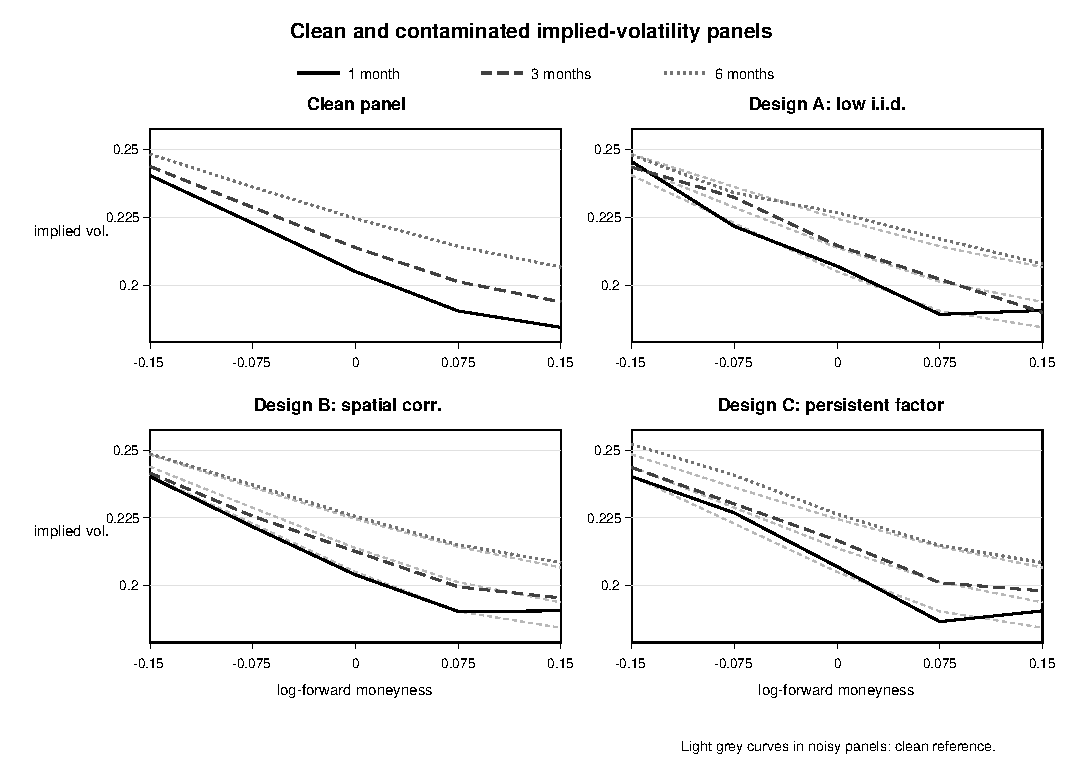
\includegraphics[width=0.95\textwidth]{figures/noise/noise_surface_comparison_sample000_date129.pdf}
    \caption{Clean and noisy implied-volatility panels for sample 000 at week index 129. The clean panel is generated exactly from the Heston pricing model. Designs A--C introduce increasingly structured quote distortions in implied-volatility space before prices are reconstructed and projected into admissible price intervals.}
    \label{fig:app_noise_surface_comparison}
\end{figure}

\begin{figure}[H]
    \centering
    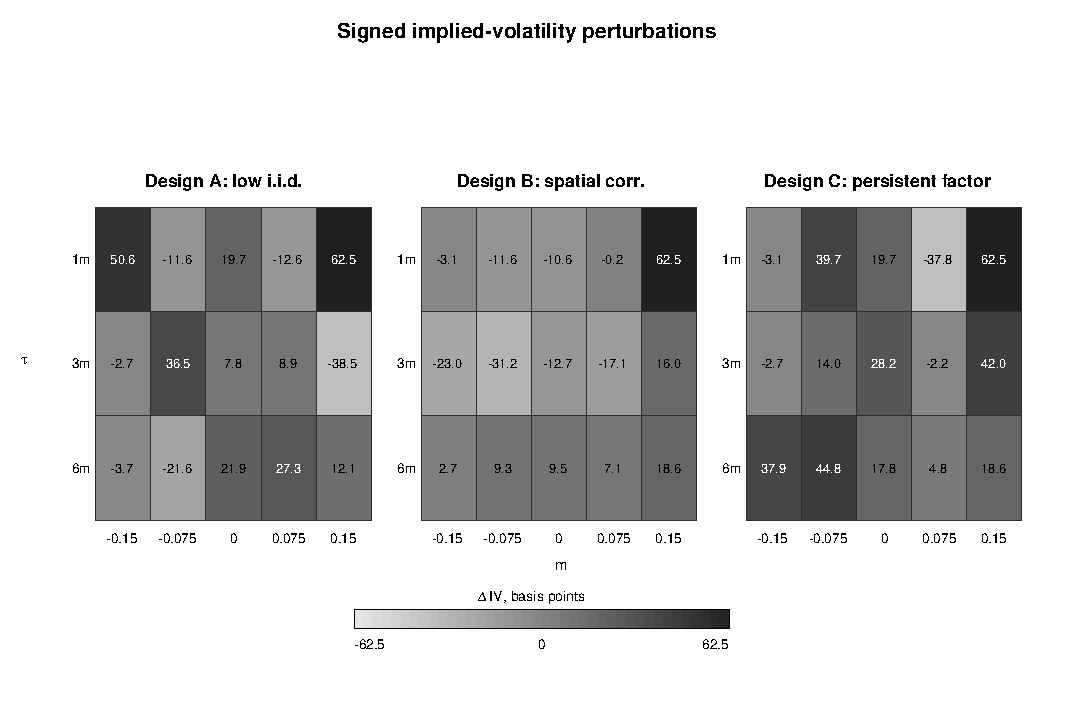
\includegraphics[width=0.9\textwidth]{figures/noise/noise_difference_comparison_sample000_date129.pdf}
    \caption{Signed implied-volatility perturbations relative to the clean model-implied panel for Designs A--C at week index 129. The plots show observed minus clean implied volatility across log-forward moneyness and maturity.}
    \label{fig:app_noise_difference_comparison}
    TODO: Re-point plot data to average sample perturbations instead of a given sample
\end{figure}

\begin{figure}[H]
    \centering
    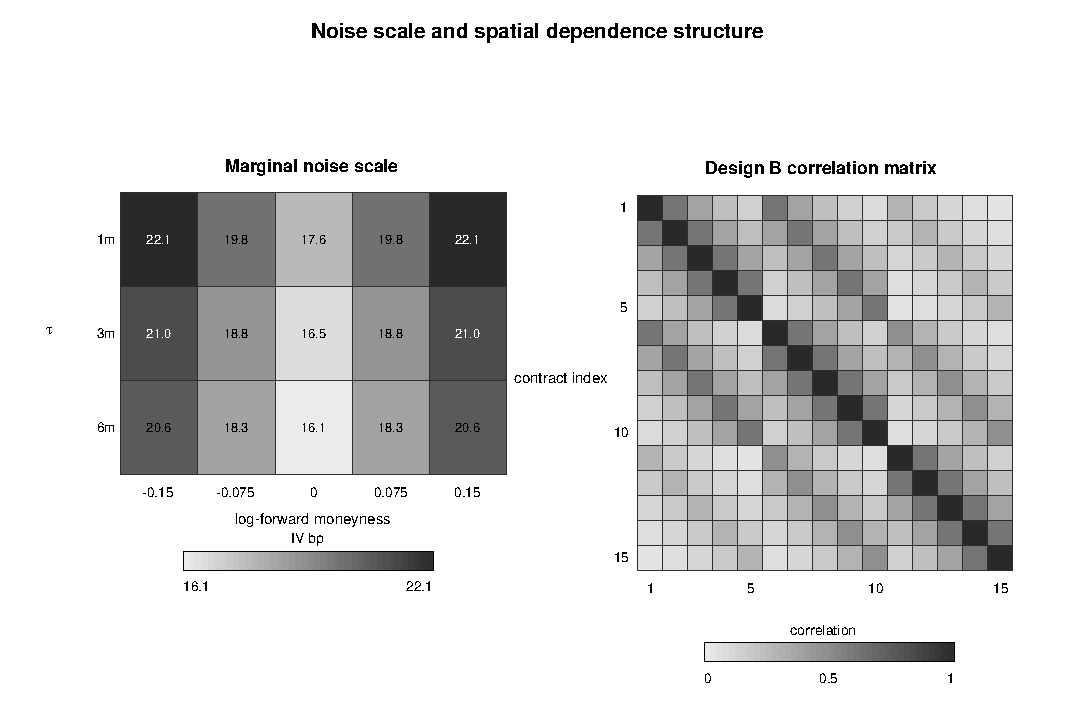
\includegraphics[width=0.9\textwidth]{figures/noise/noise_design_cross_section_structure.pdf}
    \caption{Cross-sectional structure of the observation-error designs. The left panel shows the marginal implied-volatility error scale. The right panel shows the spatial correlation matrix used in Design B after ordering contracts by maturity and log-forward moneyness.}
    \label{fig:app_noise_cross_section_structure}
\end{figure}

\begin{figure}[H]
    \centering
    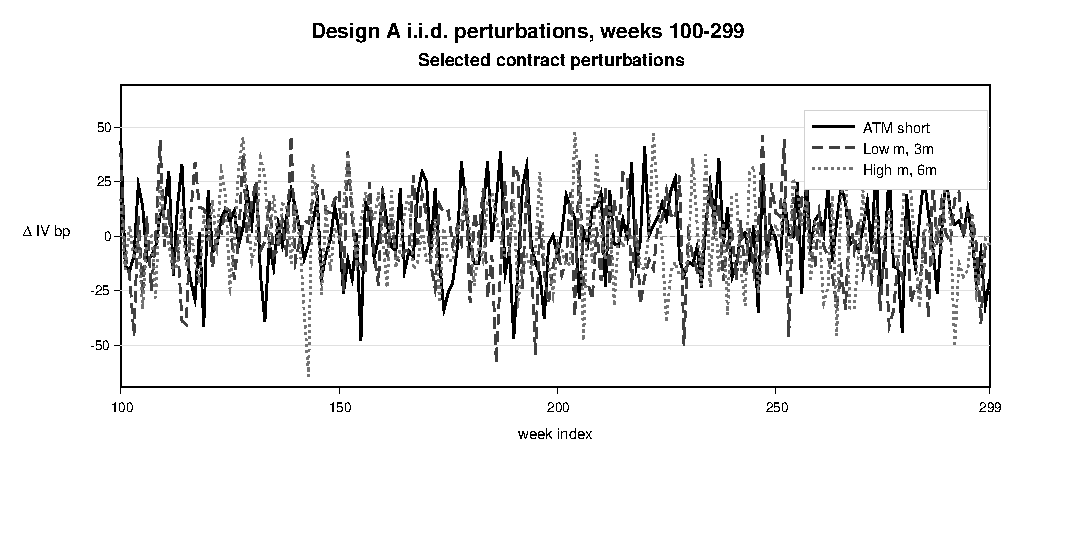
\includegraphics[width=0.9\textwidth]{figures/noise/noise_low_iid_timeseries_sample000.pdf}
    \caption{Realised perturbations for selected contracts under Design A over weeks 100--299. The series are independent across contracts conditional on the clean panel, so the plot contains no persistent common observation-error factor.}
    \label{fig:app_noise_low_iid_timeseries}
\end{figure}

\begin{figure}[H]
    \centering
    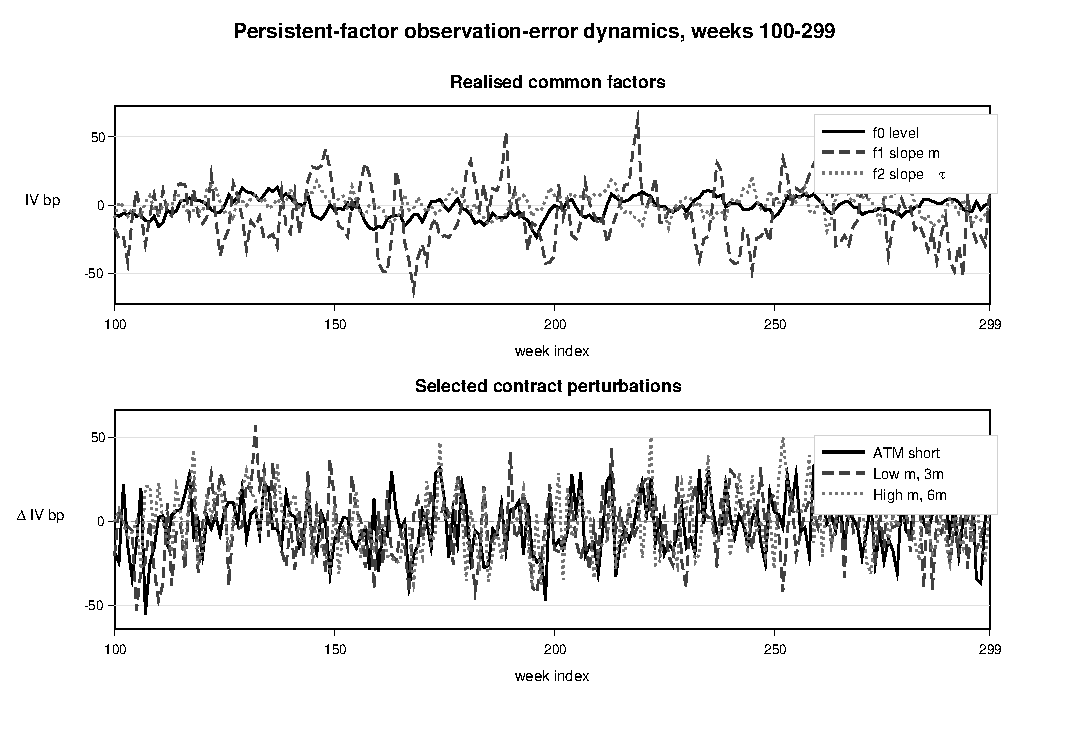
\includegraphics[width=0.95\textwidth]{figures/noise/noise_persistent_factor_timeseries_sample000.pdf}
    \caption{Temporal dependence in Design C over weeks 100--299. The upper panel shows the realised level, moneyness-slope and maturity-slope observation-error factors. The lower panel shows the resulting serially persistent implied-volatility perturbations for selected representative contracts.}
    \label{fig:app_noise_persistent_factor}
\end{figure}


\section{Implementation of the IS C-GMM Estimator}
\label{app:is_cgmm_implementation}

This appendix records the numerical implementation of the implied-state C-GMM estimator introduced in Section~\ref{sec:is_cgmm_estimation}. The purpose is to separate the computational choices needed for the Monte Carlo exercise from the main description of the estimator.

\subsection{Construction of implied variance states}

For each observation date \(t_i\), the implied-state step solves the scalar minimisation problem in \eqref{eq:is_implied_state}. The implementation uses the observed Black-Scholes implied-volatility panel as the target object. For each candidate variance value \(v\), Heston option prices are computed under \(\mathbb Q\) for all contracts in \(\mathcal C_i\), using the risk-neutral parameter subset \(\theta_{\mathbb Q}\). These model prices are then inverted into Black-Scholes implied volatilities using the same implied-volatility inversion convention as that used in the construction of the clean and noisy panels. The criterion function is the sum of squared differences between observed and model-implied volatilities across the contracts in the panel for date \(i\).

The minimisation is one dimensional because the Heston design contains a single latent variance state. The search is carried out over a bounded interval \(\mathcal V=[\underline V,\overline V]\). Consecutive option panels are close in time, so the numerical search can be "warm-started" from the previously implied variance level. In the clean-panel case, evaluating the state-implying step at the true risk-neutral parameter vector provides a direct numerical check on the implementation, since the recovered sequence should be close to the simulated variance path.

The same procedure is applied to clean and noisy option panels. Hence, differences between the implied states recovered from the different observation error designs are driven by the observation error mechanisms themselves and not by changes in the pricing or implied-volatility inversion convention.

\subsection{Heston transition characteristic function under \(\mathbb P\)}

The C-GMM moment conditions require the conditional characteristic function of the next estimation state
\[
X_{i+1}^{\theta_{\mathbb Q}}
=
\left(
R_{i+1},
\widehat V_{i+1}^{\theta_{\mathbb Q}}
\right)^\top
\]
given \(X_i^{\theta_{\mathbb Q}}\). In the Heston implementation this is evaluated using the physical-measure dynamics of the return and variance pair. Conditional on the current implied variance \(\widehat V_i^{\theta_{\mathbb Q}}\), the relevant characteristic function is written in affine form as
\[
\varphi\left(s,X_i^{\theta_{\mathbb Q}},\Delta;\theta\right)
=
\exp\left(
A(\Delta;s,\theta)
+
B(\Delta;s,\theta)
\widehat V_i^{\theta_{\mathbb Q}}
\right),
\label{eq:app_heston_transition_ccf}
\]
where \(s=(s_R,s_V)^\top\). The affine coefficients solve the Riccati system associated with the Heston dynamics under \(\mathbb P\). With terminal loading \(B(0)=is_V\), the scalar Riccati equation for \(B\) can be written as
\[
\frac{\dif B}{\dif t}
=
a+bB+cB^2,
\]
where
\[
a
=
is_R\left(\eta-\frac{1}{2}\right)
-\frac{1}{2}s_R^2,
\qquad
b
=
-\kappa+\rho\sigma_v is_R,
\qquad
c
=
\frac{1}{2}\sigma_v^2 .
\]
The corresponding \(A\) coefficient satisfies
\[
\frac{\dif A}{\dif t}
=
is_R(r-q)+\kappa\bar V B .
\]
The implementation evaluates this system using the analytic Heston Riccati solution. A Runge--Kutta solver is retained as a reference implementation and is used for numerical validation of the analytic formula. This is useful because the characteristic function contains complex square roots and logarithms, for which branch choices can otherwise become a source of numerical error.

\subsection{Evaluation of the continuum GMM criterion}

Let \(\tau=(u,s)\), where \(u\in\mathbb R^2\) denotes the instrument argument and \(s\in\mathbb R^2\) denotes the conditional characteristic function argument. The first step criterion in \eqref{eq:is_cgmm_first_step_criterion} is evaluated using an integrating density \(\pi(\tau)\). In the numerical implementation this density is chosen so that
\[
\pi(\tau)=\pi_u(u)\pi_s(s),
\]
with Gaussian weights for the instrument component. The integration over the instrument argument can then be carried out analytically. Specifically, the products of instrument functions generate terms of the form
\[
\int
\exp\left(
iu^\top
\left(
X_i^{\theta_{\mathbb Q}}
-
X_j^{\theta_{\mathbb Q}}
\right)
\right)
\pi_u(u)\,\dif u ,
\]
which reduce to a Gaussian kernel in the distance between the two implied-state observations. This leaves a finite dimensional numerical integration over the \(s\)-argument of the conditional characteristic function. The implementation uses deterministic quadrature nodes for this remaining integral.

This construction follows the same principle as in the continuum-GMM implementation of \citet{boswijk2015asset}: the criterion uses the conditional characteristic function to generate a continuum of moment restrictions, while numerical integration and analytic simplifications are used to keep the criterion evaluation computationally feasible.

\subsection{Parameter transformation and numerical minimisation}

The first-step estimator minimises \(Q_T^{(1)}(\theta)\) over the admissible parameter set \(\Theta\). In the numerical implementation, the constrained Heston parameters are mapped to an unconstrained or bounded free vector. The transformation is based on
\[
\left(
\eta,
\log\kappa,
\log\bar V,
\log\sigma_v,
\operatorname{atanh}\rho,
\log\kappa_{\mathbb Q}
\right),
\]
where
\[
\kappa_{\mathbb Q}=\kappa-\eta_V,
\qquad
\eta_V=\kappa-\kappa_{\mathbb Q}.
\]
This parameterisation enforces positivity of the mean-reversion, long-run variance, vol-of-vol and risk-neutral mean-reversion parameters, while keeping \(\rho\) inside \((-1,1)\). The criterion is deterministic for a fixed simulated panel, but it is expensive because each function evaluation requires a full reconstruction of the implied variance sequence. The implementation therefore uses derivative-free minimisation with a small number of deterministic starting points and records objective values, implied-state diagnostics and timing information.

At the present stage the Monte Carlo design uses the first-step C-GMM criterion. Efficient second-step weighting is conceptually standard in the continuum-GMM setting, but is deferred in the current implementation in order to keep the comparison with the particle-filter estimator focused on the finite-sample consequences of the state recovery step and the option-panel observation error.


%========================================================
\newpage

\bibliographystyle{apalike}
\nocite{*}
\bibliography{P_ONE_BIB}
\end{document}
